\documentclass[UTF8,a4paper,zihao=-4,fontset=fandol]{ctexart}

% -------------------- 页面与字体 --------------------
\usepackage[left=27mm,right=24mm,top=25mm,bottom=25mm,headheight=14pt]{geometry}
\usepackage{setspace}
\setstretch{1.38}
\setlength{\parindent}{2em}
\setlength{\parskip}{0pt}
\raggedbottom
\emergencystretch=2em
\clubpenalty=10000
\widowpenalty=10000
\displaywidowpenalty=10000

% -------------------- 图、表、公式 --------------------
\usepackage{graphicx}
\graphicspath{{figures/}}
\usepackage{amsmath,amssymb}
\usepackage{booktabs,tabularx,array,longtable}
\usepackage{caption}
\usepackage{float}
\usepackage[section]{placeins}
\usepackage{enumitem}
\usepackage{xcolor}

\newcolumntype{Y}{>{\raggedright\arraybackslash}X}
\newcolumntype{C}[1]{>{\centering\arraybackslash}p{#1}}
\newcolumntype{R}[1]{>{\raggedleft\arraybackslash}p{#1}}
\renewcommand{\arraystretch}{1.22}
\setlength{\tabcolsep}{5pt}

\captionsetup{
  font=small,
  labelfont=bf,
  labelsep=quad,
  justification=justified,
  singlelinecheck=false,
  skip=6pt
}
\setlength{\textfloatsep}{13pt plus 3pt minus 3pt}
\setlength{\floatsep}{12pt plus 3pt minus 3pt}
\setlength{\intextsep}{12pt plus 3pt minus 3pt}

% 让纯浮动页从页顶开始排列，避免图片在页面中间漂浮。
\makeatletter
\setlength{\@fptop}{0pt}
\setlength{\@fpsep}{13pt}
\setlength{\@fpbot}{0pt plus 1fil}
\makeatother
\renewcommand{\topfraction}{0.95}
\renewcommand{\bottomfraction}{0.90}
\renewcommand{\textfraction}{0.06}
\renewcommand{\floatpagefraction}{0.78}

% -------------------- 标题、页眉与链接 --------------------
\usepackage{fancyhdr}
\usepackage[hidelinks,unicode]{hyperref}
\urlstyle{same}

\ctexset{
  section={
    format=\Large\bfseries,
    beforeskip=1.8ex plus 0.3ex minus 0.2ex,
    afterskip=0.9ex plus 0.2ex
  },
  subsection={
    format=\large\bfseries,
    beforeskip=1.5ex plus 0.2ex minus 0.2ex,
    afterskip=0.7ex plus 0.2ex
  },
  subsubsection={
    format=\normalsize\bfseries,
    beforeskip=1.2ex plus 0.2ex minus 0.2ex,
    afterskip=0.5ex plus 0.1ex
  }
}

\pagestyle{fancy}
\fancyhf{}
\fancyhead[L]{\small 511 keV 双光子标记背散射成像系统}
\fancyhead[R]{\small 阶段性研究报告}
\fancyfoot[C]{\thepage}
\renewcommand{\headrulewidth}{0.4pt}
\renewcommand{\footrulewidth}{0pt}

\setlist[itemize]{leftmargin=2.2em,itemsep=0.2em,topsep=0.4em,parsep=0pt}
\setlist[enumerate]{leftmargin=2.4em,itemsep=0.2em,topsep=0.4em,parsep=0pt}

\begin{document}

% -------------------- 封面 --------------------
\hypersetup{pageanchor=false}
\begin{titlepage}
  \thispagestyle{empty}
  \centering
  \vspace*{0.17\textheight}
  {\zihao{1}\bfseries 511 keV 双光子标记背散射成像系统\par}
  \vspace{0.8em}
  {\zihao{1}\bfseries 的蒙特卡洛构建与性能评价\par}
  \vspace{2.2em}
  {\zihao{2}\bfseries 阶段性研究报告\par}
  \vfill
  \renewcommand{\arraystretch}{1.45}
  \begin{tabular}{rl}
    仿真环境：& vGate 9.4.1 / GATE 9.4.1 / Geant4 11.3.0 \\
    当前阶段：& 理想探测器蒙特卡洛仿真、重建与性能评价 \\
    报告日期：& 2026年7月20日 \\
  \end{tabular}
  \vspace*{0.10\textheight}
\end{titlepage}

\hypersetup{pageanchor=true}
\pagenumbering{Roman}

% -------------------- 摘要 --------------------
\section*{摘要}
\addcontentsline{toc}{section}{摘要}

为评价合理尺寸探测器的背散射成像能力，本研究构建了基于反向发射
511~keV 双光子标记的 GATE 蒙特卡洛模型，并建立了从 D1/D2 Hits 输出、
事件聚合和符合筛选到康普顿散射点重建、真值评价及图像生成的完整分析链路。
200 万初级事件的均匀水泥基线中，D2 全能峰众数为 511.5~keV，D1 能谱覆盖
$90^\circ$--$180^\circ$ 单次背散射对应的 170.33--255.50~keV 理论区域；
52 项自动测试及散射顶点闭环验证支持当前理想模型的能量、事件配对和重建正确性。
严格单次散射样本中，92.3\% 的重建深度位于实际水泥板内。深度分析表明，
目标加深会同时降低灵敏度并增大轴向误差；直径 20~mm、深度 30~mm 的水泥
孔洞在已知位置分析中达到 $\mathrm{CNR}=9.13$，随后完成的 6+6 小样本答案隔离
盲检流程亦通过。参数扫描显示，D2 部分能量沉积事件在理想条件下可使真信号
最多增加约 50\%，而轴向误差未见明显恶化；D1 外半径 150~mm 相对 200~mm
减少约 44.2\% GAGG 质量，并保留约 93.6\% 的 30~mm 薄层信号。探测器分区
结果表明，全 D1/D2 仍具有最佳综合灵敏度，D1 内侧区域和 D2 外环可作为辅助
通道。上述结果限定于理想探测器模型，仍需真实能量分辨率、触发阈值、位置
读出和更大规模盲检数据进一步验证。

\vspace{0.8em}
\noindent\textbf{关键词：}康普顿背散射成像；GATE；511~keV 双光子标记；
水泥孔洞；空间分辨率；成像灵敏度；探测器尺寸

\clearpage
\begingroup
  \small
  \setstretch{1.05}
  \setlength{\parskip}{0pt}
  \tableofcontents
\endgroup
\clearpage
\pagenumbering{arabic}

% -------------------- 正文 --------------------
\section{研究背景与目标}

背散射成像系统的性能不能由单一图像或单一分辨率数字概括。探测器几何、事件
筛选、目标深度和材料衰减会共同影响有效事件数、空间响应和缺陷对比度。因此，
本研究围绕三个相互关联的问题展开：系统的输运与重建链路是否正确；系统在
水泥等对象中能够获得怎样的深度、分辨率和缺陷信号；探测器尺寸及不同区域的
使用方式如何影响灵敏度与成像质量。

研究采用 D1 背散射成像探测器与 D2 标记/准直探测器。放射源发射两个方向相反
的 511~keV 光子：一个光子由 D2 提供时间和方向标记，另一个光子进入被测物体，
经康普顿散射后由 D1 接收。D1 沉积能量与 D1/D2 探测位置共同用于求解散射点。
本阶段建立并检查了以下数据链：

\begin{center}
  \small
  \fbox{\parbox{0.92\linewidth}{\centering
  GATE 光子输运 $\rightarrow$ D1/D2 探测器 Hits $\rightarrow$ 事件聚合
  $\rightarrow$ 双光子符合 $\rightarrow$ 事件筛选\\
  $\rightarrow$ 散射点重建 $\rightarrow$ 仿真真值评价 $\rightarrow$ 图像和性能指标}}
\end{center}

本阶段已覆盖均匀水泥、不同深度薄层、细杆、双杆、边缘和水泥孔洞体模，并对
D1/D2 能量窗、角度范围、D1 尺寸以及 D1/D2 分区进行了扫描。水（Water）和
铁（Iron）已完成同条件配置，但尚未形成正式大样本结果。因此，本文重点报告
水泥对象和理想探测器条件下的阶段性证据，不将其外推为实际硬件的最终性能。

\section{仿真系统与研究方法}

\subsection{几何和部件}

\begin{table}[htbp]
  \centering
  \caption{仿真系统的主要几何与部件设置}
  \label{tab:geometry}
  \small
  \begin{tabularx}{\linewidth}{@{}p{0.12\linewidth}Y Y@{}}
    \toprule
    部件 & 当前设置 & 作用 \\
    \midrule
    放射源 & 位于 $(0,0,17.5)~\mathrm{mm}$，每次发射两个方向相反的 511~keV 光子
      & 提供标记光子和入射物体的光子 \\
    D1 & GAGG 环，内/外半径 20/200~mm，厚 15~mm
      & 背散射成像探测器，接收物体散射回来的光子 \\
    D2 & $50\times50$ GAGG 阵列，晶体 $0.93\times0.93\times20~\mathrm{mm^3}$，节距 1.00~mm
      & 标记/准直探测器，给出另一侧光子的时间和大致方向 \\
    水泥板 & $500\times500\times100~\mathrm{mm^3}$，深度 0--100~mm
      & 基线被测物体 \\
    坐标 & 水泥上表面为深度 0~mm，向水泥内部深度增加
      & 统一所有重建和真值口径 \\
    \bottomrule
  \end{tabularx}
\end{table}

\subsection{基线筛选条件}

\begin{itemize}
  \item D1 能量：170.34--300~keV；
  \item D2 能量：450--560~keV；
  \item 符合时间窗：10~ns；
  \item 入射角：$0^\circ$--$45^\circ$；
  \item 背散射角：$90^\circ$--$180^\circ$；
  \item D1 有效半径：20--200~mm；
  \item D2 使用完整阵列。
\end{itemize}

这些条件只使用实验中能够测量的能量、时间和探测器位置。GATE 提供的
\texttt{nPhantomCompton}、材料名称和真实散射顶点只用于事后评分，不参与
实际选事件。

\subsection{仿真与分析流程}

GATE 端负责：

\begin{enumerate}
  \item 建立放射源、D1、D2 和水泥几何；
  \item 运输 511~keV 光子；
  \item 输出 D1、D2 的 Hits ROOT；
  \item 记录水泥中的康普顿次数、散射材料和真实散射顶点。
\end{enumerate}

Windows/Python 端负责：

\begin{enumerate}
  \item 把同一次 GATE 事件中的多个 Hit 聚合为探测器事件；
  \item 按 \texttt{(runID,eventID)} 配对 D1 和 D2；
  \item 按时间、能量、角度和探测器区域筛选；
  \item 使用 D1 能量和 D1/D2 位置求康普顿散射点；
  \item 用仿真真值计算偏差、RMSE、FWHM、灵敏度和纯度；
  \item 导出 PNG、SVG、PDF、TIFF、CSV 和 JSON。
\end{enumerate}

\subsection{标准体模与评价指标}

均匀水泥板用于检查完整成像链路、深度分布和单位初级事件灵敏度；真空环境中的
1~mm 水泥薄层用于测量轴向本征响应；实体水泥单杆、双杆和边缘体模用于评价
横向 FWHM、双峰可分辨性和调制传递函数（MTF）；完整水泥板中的圆柱形真空区
用于近似空气孔洞，并以对比度、对比噪声比（CNR）及答案隔离盲检评价缺陷信号。
其中双杆是位于真空中的实体水泥圆柱，不等同于水泥内部的杆状孔洞。

灵敏度统一定义为每 $10^6$ 个初级事件得到的有效成像事件数。轴向响应以薄层
误差分布的半高全宽（FWHM）和逐事件 $z$ 均方根误差（RMSE）评价；横向分辨
能力使用细杆 FWHM、双杆谷峰比和边缘 MTF 评价。均匀水泥本身具有有限厚度，
因此其整体重建分布宽度不作为系统分辨率。

\section{系统正确性与能谱验证}

\subsection{基线数据规模}

正式完整水泥基线使用 2,000,000 个初级事件，得到表~\ref{tab:baseline-counts}
所示数据规模。

\begin{table}[htbp]
  \centering
  \caption{完整水泥基线的数据规模}
  \label{tab:baseline-counts}
  \begin{tabular}{@{}lr@{}}
    \toprule
    数据级别 & 数量 \\
    \midrule
    D1 聚合事件 & 587,238 \\
    D2 聚合事件 & 909,751 \\
    同一 GATE 事件中的 D1/D2 配对 & 284,652 \\
    可观测筛选后有效重建 & 52,979 \\
    匹配到水泥真值的有效重建 & 52,071 \\
    严格单次水泥康普顿有效重建 & 27,956 \\
    \bottomrule
  \end{tabular}
\end{table}

\subsection{D1/D2 能谱}

\begin{figure}[htbp]
  \centering
  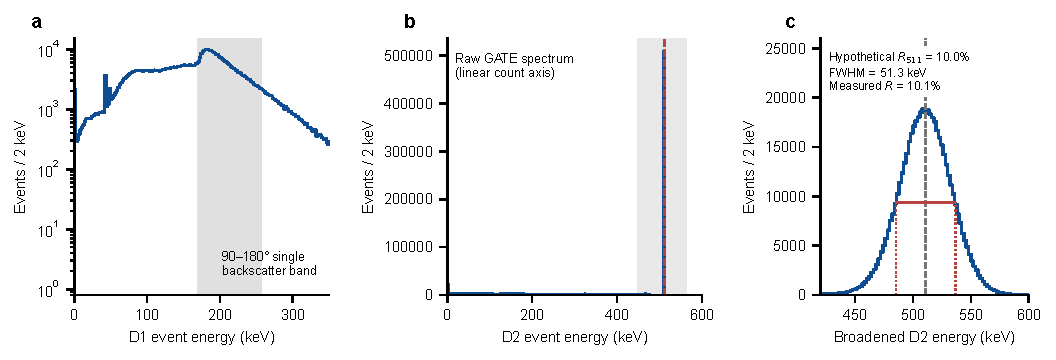
\includegraphics[width=0.98\linewidth]{fig01_energy_spectra.pdf}
  \caption{D1 和 D2 正式能谱，以及 D2 假设能量展宽。a，D1 原始聚合能谱，
  灰色区域为 511~keV 光子在 $90^\circ$--$180^\circ$ 单次背散射后的理论能量带。
  b，D2 原始能谱采用普通线性计数坐标；511~keV 尖峰远高于连续谱，因此连续谱
  看起来接近横轴。c，假设 $10\%~\mathrm{FWHM}@511~\mathrm{keV}$ 后的 D2
  展宽峰，并标出半高宽。}
  \label{fig:energy-spectra}
\end{figure}

\subsection{多层一致性验证}

目前有五层相互独立的正确性证据：

\begin{enumerate}
  \item \textbf{源能量正确：}D2 全能峰众数为 511.5~keV，与设置的 511~keV
  标记光子一致。0.5~keV 的差别来自 1~keV 统计箱中心。
  \item \textbf{背散射能量正确：}511~keV 光子在 $90^\circ$--$180^\circ$
  单次康普顿散射后的理论光子能量为 170.33--255.50~keV，D1 能谱覆盖该区域。
  \item \textbf{复杂过程符合预期：}D1 理论带外仍有部分沉积、多次散射和
  非目标过程，没有把所有事件强行裁剪进理论区间。
  \item \textbf{重建公式闭环：}人工合成的已知散射顶点可被闭式公式恢复，
  最大数值误差为 $6.49\times10^{-12}~\mathrm{mm}$；运动学不可能的事件会被拒绝。
  \item \textbf{真实 GATE 顶点闭环：}重建点能够与 PhaseSpaceActor 记录的
  真实康普顿顶点匹配，并计算偏差和 RMSE。
\end{enumerate}

图~\ref{fig:energy-spectra}c 的能量分辨率定义为

\begin{equation}
  R=\frac{\mathrm{FWHM}}{E_{\mathrm{peak}}}.
  \label{eq:energy-resolution}
\end{equation}

输入假设为 10.0\%，展宽直方图测得 $\mathrm{FWHM}=51.3~\mathrm{keV}$、
$R=10.1\%$。这里的 10\% 是展示和敏感性分析情景，不是实测 GAGG/SiPM 标定值。

\subsection{本节小结与证据边界}

D2 全能峰与 511~keV 源能一致，D1 能谱覆盖理论单次背散射区间，重建公式和
GATE 真值均完成闭环检查，因此当前理想模型的能量、事件配对和散射点求解链路
通过一致性验证。该结论不等同于真实探测器实验验证；图~\ref{fig:energy-spectra}c
采用的 10\% 能量分辨率是明确的情景假设，而不是 GAGG/SiPM 实测标定值；
D1 理论带外计数则包含部分能量沉积、多次散射和非目标过程，不能简单归为程序错误。

\section{水泥对象的成像性能}

\subsection{均匀水泥板重建}

\begin{figure}[htbp]
  \centering
  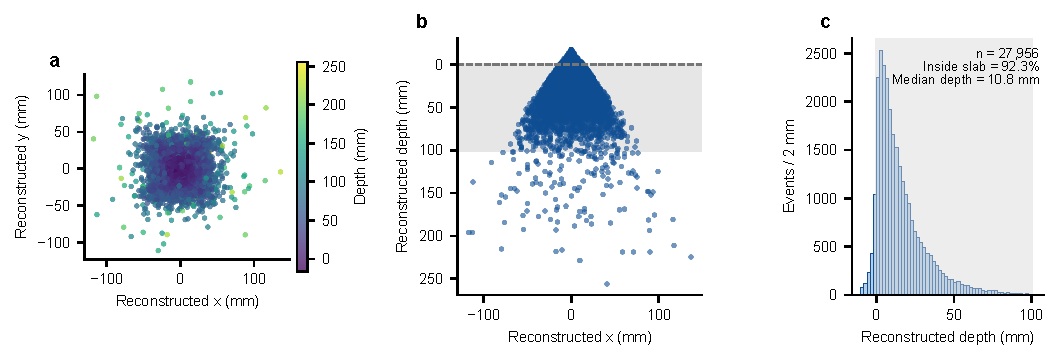
\includegraphics[width=0.98\linewidth]{fig02_reconstruction_distribution.pdf}
  \caption{完整水泥板的重建分布。a，横向重建点；b，横向--深度分布，灰色
  区域为实际水泥范围；c，重建深度分布。27,956 个严格单次散射事件中，
  92.3\% 的重建深度落在水泥板内。该图用于证明成像链路工作，不能把均匀
  水泥分布宽度称为系统分辨率。}
  \label{fig:reconstruction-distribution}
\end{figure}

完整水泥板的严格单次散射结果为：

\begin{itemize}
  \item 整体 $z$ 偏差：$-1.12~\mathrm{mm}$；
  \item 整体 $z$ RMSE：11.68~mm；
  \item 3D RMSE：13.12~mm；
  \item 重建深度落在水泥板内：92.3\%。
\end{itemize}

\subsection{水泥中的成像深度、灵敏度和模糊程度}

\begin{figure}[htbp]
  \centering
  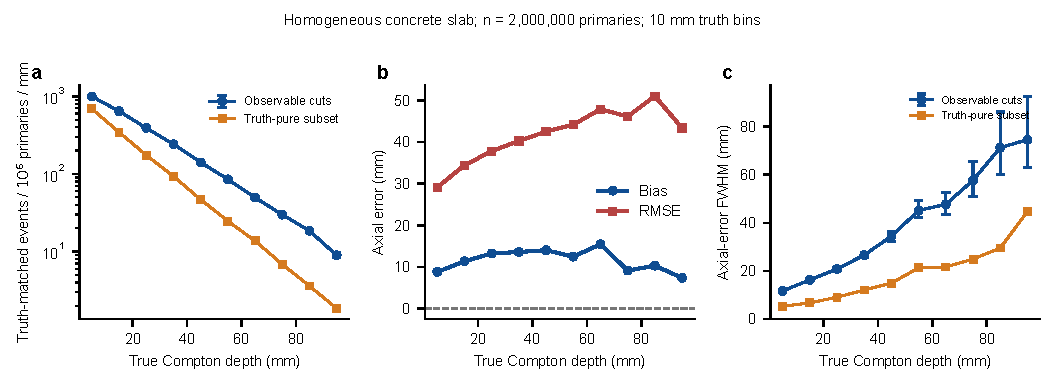
\includegraphics[width=0.98\linewidth]{fig03_concrete_depth_profile.pdf}
  \caption{完整水泥板内的深度性能。a，深度越大，单位初级事件留下的信号越少；
  b，偏差和逐事件 RMSE；c，轴向误差 FWHM，误差棒为统计区间。蓝色表示可观测
  筛选结果，橙色为事后真值纯子集。}
  \label{fig:concrete-depth}
\end{figure}

代表性深度结果见表~\ref{tab:depth-results}。

\begin{table}[htbp]
  \centering
  \caption{完整水泥板中的代表性深度性能}
  \label{tab:depth-results}
  \begin{tabular}{@{}ccc@{}}
    \toprule
    真实深度 & 灵敏度（事件/$10^6$ 初级/mm） & 可观测误差 FWHM \\
    \midrule
    0--10~mm  & 995.95 & 11.68~mm \\
    20--30~mm & 390.65 & 20.85~mm \\
    30--40~mm & 241.50 & 26.63~mm \\
    50--60~mm & 85.30  & 45.16~mm \\
    90--100~mm & 8.95  & 74.59~mm \\
    \bottomrule
  \end{tabular}
\end{table}

因此，“成像深度”不能脱离允许的模糊程度单独报告：

\begin{itemize}
  \item 以 $\mathrm{FWHM}\leq20~\mathrm{mm}$ 为判据：本批数据的实用深度约 20~mm；
  \item 以 $\mathrm{FWHM}\leq30~\mathrm{mm}$ 为判据：约 40~mm；
  \item 以 $\mathrm{FWHM}\leq50~\mathrm{mm}$ 为判据：约 70~mm。
\end{itemize}

这些数字依赖本次 200 万事件和当前统计门槛，不是与采集时间无关的绝对穿透深度。

\subsection{水泥孔洞成像}

在 $500\times500\times100~\mathrm{mm^3}$ 水泥板中加入圆柱形真空区，近似
空气孔洞。四组条件为直径 10/20~mm、中心深度 30/60~mm，每组 200 万初级事件。

\begin{figure}[htbp]
  \centering
  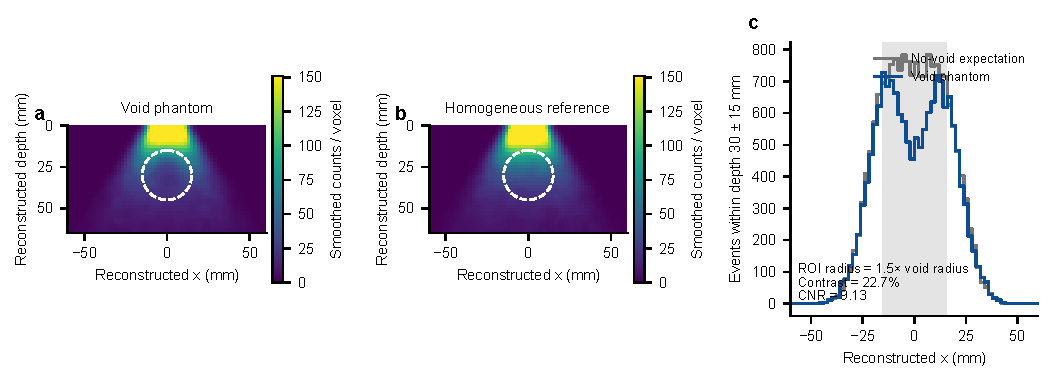
\includegraphics[width=0.98\linewidth]{fig04_concrete_void_detectability.pdf}
  \caption{直径 20~mm、中心深度 30~mm 的水泥孔洞成像。a，含孔洞水泥的
  重建图；b，均匀水泥参照；c，孔洞深度附近的横向计数分布。该条件对比度为
  22.7\%，CNR 为 9.13。}
  \label{fig:void-detectability}
\end{figure}

\begin{table}[htbp]
  \centering
  \caption{四组水泥孔洞的已知位置分析结果}
  \label{tab:void-results}
  \begin{tabular}{@{}ccccc@{}}
    \toprule
    孔洞直径 & 中心深度 & 对比度 & CNR & 当前判断 \\
    \midrule
    10~mm & 30~mm & 12.9\% & 2.38 & 弱证据 \\
    10~mm & 60~mm & 12.1\% & 1.42 & 弱证据 \\
    20~mm & 30~mm & 22.7\% & 9.13 & 已知位置下明显 \\
    20~mm & 60~mm & 4.3\%  & 0.98 & 本次不能可靠看见 \\
    \bottomrule
  \end{tabular}
\end{table}

为了避免“知道孔洞位置后再挑区域”，又完成了 12 例答案隔离盲检流程验收。

\begin{figure}[htbp]
  \centering
  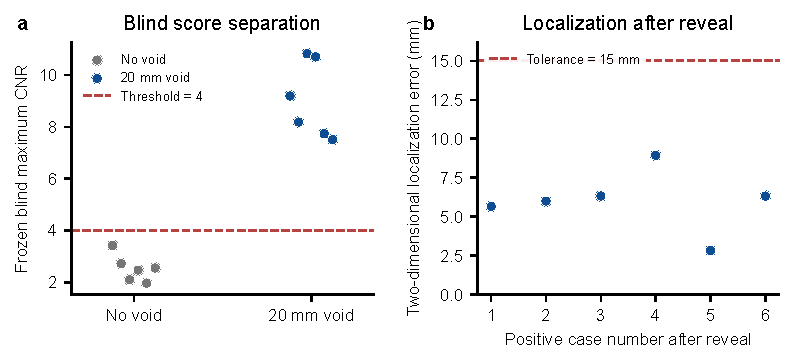
\includegraphics[width=0.88\linewidth]{fig05_blind_qualification_summary.pdf}
  \caption{水泥孔洞小样本盲检流程验收。左，6 个无孔洞样本分数均低于冻结
  阈值 4，6 个孔洞样本均高于阈值；右，6 个孔洞样本揭盲后的定位误差均小于
  15~mm。}
  \label{fig:blind-qualification}
\end{figure}

正确结论是“6+6 小样本盲检流程验收通过”，不能写成已经确定了 100\% 检出率
和 0\% 误报率，因为相应 95\% 区间仍很宽。

\subsection{本节小结}

水泥对象的数据生成、均匀介质重建、深度性能、孔洞成像和小样本盲检流程均
已完成。水和铁的正式 200 万事件材料对比尚未运行，因此“不同物体”目前以
不同水泥标准体模和水泥孔洞为主，现有证据尚不足以支持跨材料泛化结论。

\section{事件筛选、探测器尺寸与空间分辨特性}

\subsection{评价原则}

每次只改变一个筛选条件，并同时观察：

\begin{itemize}
  \item 灵敏度：能留下多少有效信号；
  \item 纯度：留下的事件中真目标事件占多少；
  \item 分辨率或误差：FWHM、RMSE、双峰可分辨性或 MTF；
  \item 稳健性：结果是否依赖分箱、平滑带宽或随机种子。
\end{itemize}

不能只选择“让峰最窄”的窗口，因为很窄的窗口可能把绝大多数信号都删掉。

\subsection{D1 能量窗}

以 30~mm 薄层标准目标为例，筛选结果见表~\ref{tab:d1-window}。

\begin{table}[htbp]
  \centering
  \caption{D1 能量窗对真目标事件保留率和轴向响应的影响}
  \label{tab:d1-window}
  \begin{tabular}{@{}ccc@{}}
    \toprule
    D1 能窗 & 真目标事件保留 & 轴向 FWHM \\
    \midrule
    170.34--300~keV 基线 & 100.0\% & 12.39~mm \\
    180--250~keV & 81.3\% & 10.01~mm \\
    190--240~keV & 55.4\% & 9.50~mm \\
    \bottomrule
  \end{tabular}
\end{table}

收窄 D1 能窗能使核心响应变窄，但会牺牲灵敏度。180--250~keV 是当前较平衡
的候选，最终仍应带入孔洞 CNR 决定。

\subsection{D2 部分能量事件的接受范围}

D2 能量当前只用于决定事件是否接收，没有直接代入散射点求解。因此光子在 D2
中部分沉积能量后逃逸的事件仍可能提供有用的时间和位置标记。

\begin{figure}[htbp]
  \centering
  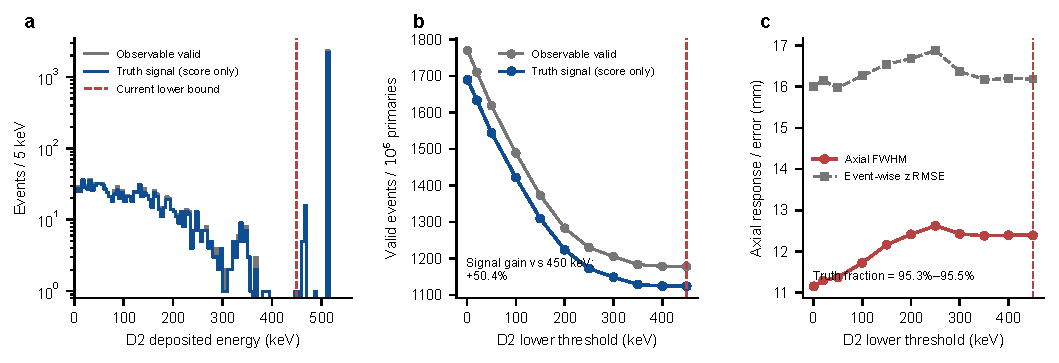
\includegraphics[width=0.98\linewidth]{fig06_d2_energy_acceptance.pdf}
  \caption{D2 能量下限与灵敏度和轴向误差。a，完成其他筛选后仍存在的 D2
  部分能量事件；b，降低 D2 下限会增加有效信号；c，轴向 FWHM、$z$ RMSE 和
  真信号比例。红色虚线为原基线 450~keV。}
  \label{fig:d2-energy}
\end{figure}

\begin{table}[htbp]
  \centering
  \caption{D2 能量下限对真信号和轴向响应的影响}
  \label{tab:d2-window}
  \small
  \begin{tabular}{@{}ccccc@{}}
    \toprule
    D2 能窗 & 真信号/$10^6$ 初级 & 相对基线增益 & 真信号占比 & 轴向 FWHM \\
    \midrule
    450--560~keV & 1,123.5 & 基线   & 95.4\% & 12.39~mm \\
    150--560~keV & 1,309.0 & $+16.5\%$ & 95.3\% & 12.16~mm \\
    50--560~keV  & 1,544.5 & $+37.5\%$ & 95.4\% & 11.37~mm \\
    1--560~keV   & 1,690.0 & $+50.4\%$ & 95.5\% & 11.15~mm \\
    \bottomrule
  \end{tabular}
\end{table}

完整水泥板也得到最多 50.7\% 的严格真信号增益，$z$ RMSE 没有恶化。
但 1~keV 是不含电子学噪声的理想边界，不是现实推荐。正式基线暂时仍保留
450--560~keV，待实测触发阈值后重点比较 50、150 和 450~keV 下限。

\subsection{入射角和散射角}

\begin{itemize}
  \item 把入射角从 $0^\circ$--$45^\circ$ 缩到 $0^\circ$--$30^\circ$，
  只保留 73.3\% 信号，FWHM 从 12.39~mm 变差为 13.30~mm；
  \item 缩到 $0^\circ$--$20^\circ$，只保留 34.1\%，FWHM 变为 15.13~mm；
  \item 因此当前几何下不建议仅凭“角度越窄越好”收紧入射角。
\end{itemize}

散射角和能量窗同样存在“响应核心变窄--信号减少”的权衡，需要和灵敏度共同看。

\subsection{D1 尺寸与成像灵敏度}

灵敏度定义为

\begin{equation}
  S(R)=\frac{N_{\mathrm{selected,valid}}(R)}{N_{\mathrm{primaries}}}.
  \label{eq:sensitivity}
\end{equation}

\begin{figure}[htbp]
  \centering
  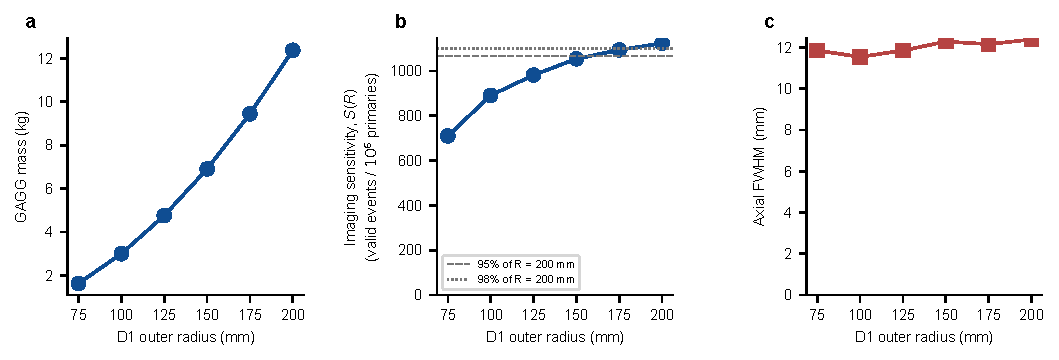
\includegraphics[width=0.98\linewidth]{fig07_d1_size_tradeoff.pdf}
  \caption{D1 尺寸、质量、灵敏度和分辨率关系。a，D1 GAGG 质量随外半径增加；
  b，成像灵敏度随半径增加后逐渐饱和；c，30~mm 薄层轴向 FWHM 基本稳定。
  虚线表示 200~mm 灵敏度的 95\% 和 98\%。}
  \label{fig:d1-size}
\end{figure}

\begin{table}[htbp]
  \centering
  \caption{D1 外半径与质量、灵敏度和轴向响应的关系}
  \label{tab:d1-size}
  \small
  \begin{tabular}{@{}ccccc@{}}
    \toprule
    D1 外半径 & GAGG 质量 & 灵敏度（事件/$10^6$ 初级） & 相对 200~mm 信号保留 & FWHM \\
    \midrule
    100~mm & 3.00~kg  & 891.0   & 79.3\% & 11.55~mm \\
    125~mm & 4.76~kg  & 981.5   & 87.4\% & 11.85~mm \\
    150~mm & 6.90~kg  & 1,054.0 & 93.8\% & 12.29~mm \\
    175~mm & 9.44~kg  & 1,093.5 & 97.3\% & 12.16~mm \\
    200~mm & 12.37~kg & 1,123.5 & 100.0\% & 12.39~mm \\
    \bottomrule
  \end{tabular}
\end{table}

后处理预测已经由真实改变 GATE 几何的 $R=150/175~\mathrm{mm}$ 仿真验证。
$R=150~\mathrm{mm}$ 薄层信号实测保留约 93.6\%，同时减少约 44.2\% GAGG
质量，因此是当前理想几何中优先评估的轻量化候选。图~\ref{fig:d1-size}中的
曲线连接六个离散采样点，用于描述经验关系，并非已经拟合和验证的连续解析函数。

\subsection{综合权衡图}

\begin{figure}[htbp]
  \centering
  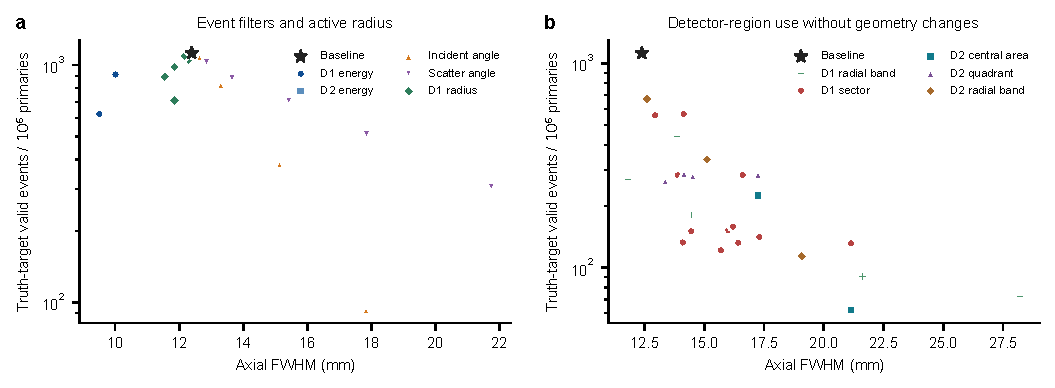
\includegraphics[width=0.98\linewidth]{fig08_sweep_tradeoffs.pdf}
  \caption{筛选条件和探测器区域的分辨率--灵敏度权衡。横坐标越小表示轴向
  FWHM 越好，纵坐标越高表示灵敏度越高，理想候选应靠近左上方。a，能量、
  角度和 D1 半径；b，不改几何时使用不同探测器区域。}
  \label{fig:sweep-tradeoffs}
\end{figure}

图~\ref{fig:sweep-tradeoffs}说明不存在一个在所有指标上都最好的筛选条件。
任何“优化”都必须同时报告事件数和分辨率，不能只汇报某一个更好看的数字。

\subsection{空间分辨特性}

\subsubsection{轴向本征响应}

\begin{figure}[htbp]
  \centering
  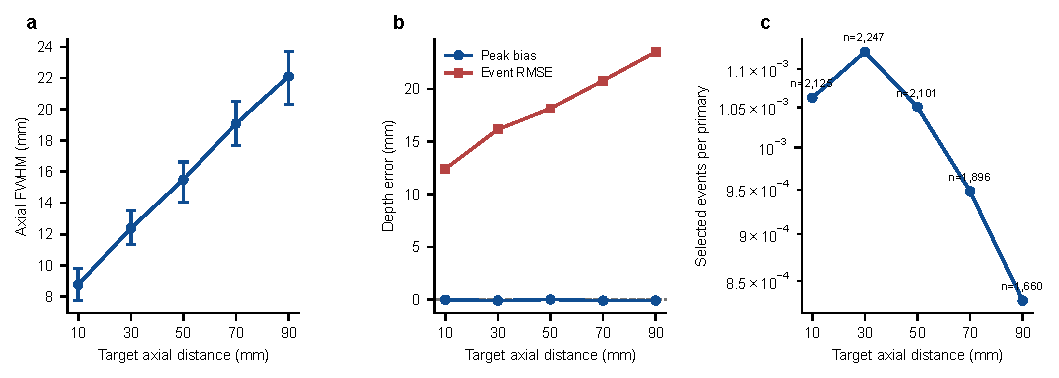
\includegraphics[width=0.98\linewidth]{fig09_depth_performance.pdf}
  \caption{不同轴向距离的薄层响应。真空中 1~mm 水泥薄层从 10~mm 移到
  90~mm 后，轴向 FWHM 由 8.77~mm 增至 22.11~mm。该图测量理想几何响应，
  不代表完整水泥中的穿透深度。}
  \label{fig:axial-response}
\end{figure}

\begin{table}[htbp]
  \centering
  \caption{不同轴向距离的薄层轴向响应}
  \label{tab:axial-response}
  \begin{tabular}{@{}cc@{}}
    \toprule
    目标轴向距离 & 轴向 FWHM \\
    \midrule
    10~mm & 8.77~mm \\
    30~mm & 12.39~mm \\
    50~mm & 15.49~mm \\
    70~mm & 19.09~mm \\
    90~mm & 22.11~mm \\
    \bottomrule
  \end{tabular}
\end{table}

\subsubsection{横向细杆、双目标和 MTF}

\begin{itemize}
  \item 30~mm 深度的 1/2/5~mm 单杆横向 $x$ FWHM 分别为
  4.43/3.49/4.59~mm；其中 1~mm 杆只有 88 个有效事件，统计不足；
  \item 真空背景中的直径 2~mm 实体水泥双杆在中心距 5~mm 时为临界，
  10/15~mm 在三种平滑带宽下均稳定可分辨；
  \item 边缘体模在 30/70~mm 深度的模型化 MTF50 为
  0.0491/0.0263~cycles/mm，MTF10 为 0.0895/0.0480~cycles/mm。
\end{itemize}

\begin{figure}[htbp]
  \centering
  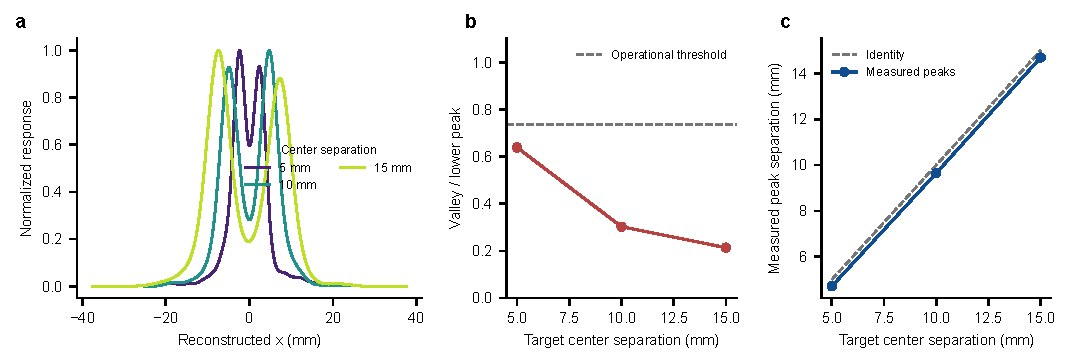
\includegraphics[width=0.98\linewidth]{fig10_double_rod_separation.pdf}
  \caption{双杆可分辨性。该体模由真空背景中的两根实体水泥圆柱组成，用于
  测量理想本征横向双目标响应，并不等同于完整水泥中的杆状孔洞。5~mm 中心距
  的谷峰比对平滑带宽敏感；10 和 15~mm 均能稳定形成双峰。因此，当前最小已
  测试的带宽稳健可分辨中心距为 10~mm。}
  \label{fig:double-rod}
\end{figure}

\begin{figure}[htbp]
  \centering
  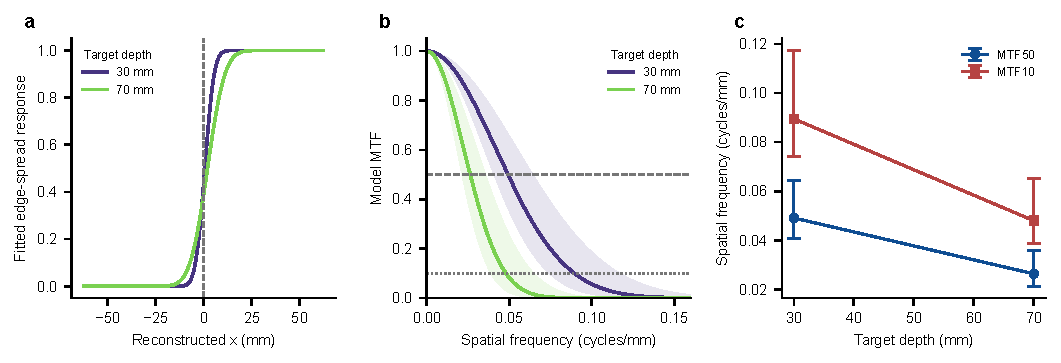
\includegraphics[width=0.98\linewidth]{fig11_edge_depth_series.pdf}
  \caption{不同深度的边缘 MTF。70~mm 深度的 MTF50 和 MTF10 均下降到
  30~mm 结果的约 54\%，说明深度增加会降低横向细节保持能力。}
  \label{fig:edge-mtf}
\end{figure}

\subsection{本节小结}

能量、角度、D1 尺寸和探测器区域对灵敏度、纯度和分辨率的理想模型影响已经
得到。最终事件窗口仍需加入实测能量分辨率、低能噪声和触发阈值，并用水泥
孔洞 CNR/盲检而不是只用薄层 FWHM 冻结。

\section{探测器分区成像}

这部分没有修改任何 GATE 几何，只在同一批原始事件中选择不同 D1/D2 区域。

\subsection{D1 不同径向区域和方位扇区}

\begin{figure}[htbp]
  \centering
  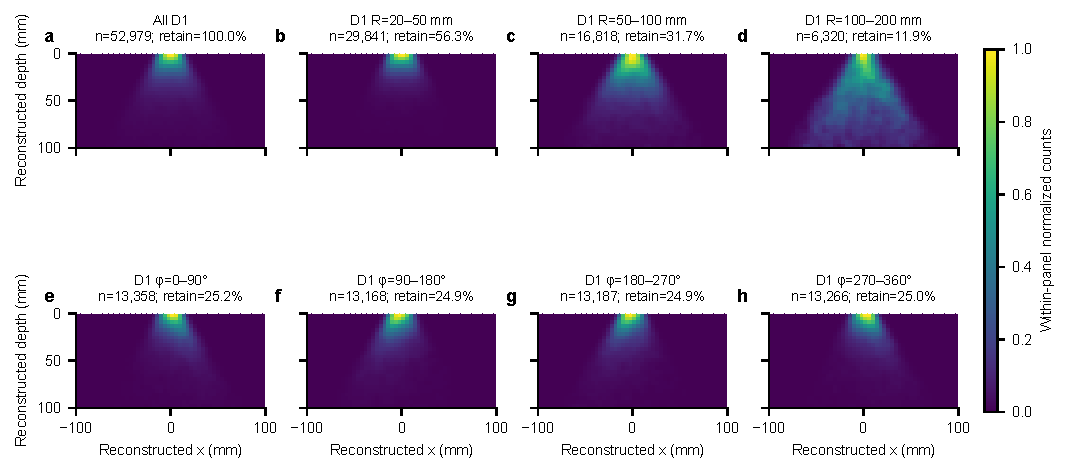
\includegraphics[width=0.98\linewidth]{fig12_d1_region_images.pdf}
  \caption{使用 D1 不同区域形成的水泥重建图。上排分别使用完整 D1、20--50、
  50--100 和 100--200~mm 径向区域；下排使用四个 $90^\circ$ 方位扇区。
  每个面板为了比较形状而单独归一化，不能通过颜色亮度比较绝对灵敏度，事件数
  和保留率写在标题中。}
  \label{fig:d1-regions}
\end{figure}

主要结果如下：

\begin{itemize}
  \item D1 20--50~mm：保留完整可观测事件的 56.3\%；
  \item D1 50--100~mm：保留 31.7\%；
  \item D1 100--200~mm：保留 11.9\%，深度分布明显更宽；
  \item 四个 $90^\circ$ 扇区各保留约 25\%，本批次总计数近似方位对称。
\end{itemize}

\subsection{D2 中心区和外环}

\begin{figure}[htbp]
  \centering
  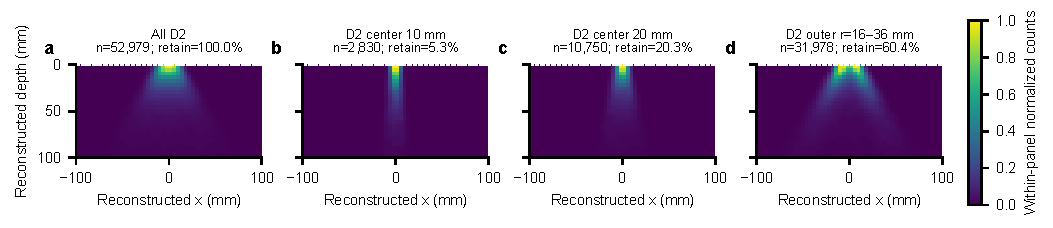
\includegraphics[width=0.98\linewidth]{fig13_d2_region_images.pdf}
  \caption{使用 D2 不同区域形成的水泥重建图。完整 D2、中心 10~mm、中心
  20~mm 和 16--36~mm 外环分别成像。只用中心区域时事件数明显下降；外环
  保留更多信号，但横向形状会改变。}
  \label{fig:d2-regions}
\end{figure}

主要结果如下：

\begin{itemize}
  \item D2 中心 10~mm：只保留 5.3\% 可观测事件；
  \item D2 中心 20~mm：保留 20.3\%；
  \item D2 16--36~mm 外环：保留 60.4\%；
  \item 30~mm 薄层中，D2 外环轴向 FWHM 为 12.61~mm；
  \item D2 中心 20/10~mm 的 FWHM 分别变差为 17.25/21.15~mm。
\end{itemize}

\subsection{本节小结}

\begin{enumerate}
  \item 全 D1、全 D2 用作主成像，综合灵敏度最好；
  \item D1 内侧径向区和 D2 外环可作为辅助重建、质量控制或多通道比较；
  \item 不推荐只使用 D2 中心区域作为主通道；
  \item 单扇区之间的小差异还需独立随机种子确认，不能立即解释成真实方位不对称。
\end{enumerate}

\section{讨论}

\subsection{主要结果的物理与工程含义}

多层一致性验证表明，当前模型已经形成从源能量、D1/D2 事件配对到康普顿
散射点求解的闭环。能谱符合理论运动学只是必要条件；合成顶点恢复、GATE 真值
匹配和自动测试共同降低了“能谱看似正确但重建链路仍存在错误”的风险。

完整水泥结果说明，成像深度、灵敏度和空间模糊不能彼此分离。深部事件需要
经历更长的入射与返回路径，因而有效计数减少、误差增大。由此得到的实用深度
必须同时给出采集统计量和允许的 FWHM 门槛，不能以“仍有少量事件”作为唯一
判据。薄层、细杆、双杆和边缘体模提供的是理想本征空间响应；水泥孔洞的 CNR
与盲检则更接近缺陷检出问题，两类指标不能相互替代。

参数扫描揭示了清晰度与计数效率之间的基本权衡。收窄 D1 能窗能够减小响应
核心宽度，但会删除一部分有效信号。D2 能量不直接进入当前散射点公式，因此
部分能量沉积事件仍可能提供时间和位置标记；理想仿真中的信号增益支持继续
研究低能窗口，但不能替代真实电子学阈值和噪声测试。D1 尺寸结果同样表现出
边际收益递减：$R=150~\mathrm{mm}$ 并非灵敏度最高的方案，而是在当前几何下
以约 6\% 信号代价换取约 44\% GAGG 减重的工程候选。若设计判据要求保留至少
95\% 的 $R=200~\mathrm{mm}$ 信号，则当前采样点中应选择 $R=175~\mathrm{mm}$，
而不是 $R=150~\mathrm{mm}$。

分区成像进一步表明，不同探测器区域提供不同的角度接受信息，但单独使用局部
区域通常会降低统计量。D2 中心图在独立归一化后看起来较窄，并不代表分辨率
更好；薄层 FWHM 的定量结果反而显示其轴向响应变差。全 D1/D2 因而仍适合作为
主成像通道，D1 内侧区域和 D2 外环更适合作为辅助重建或质量控制通道。

\subsection{阶段性研究覆盖范围}

\begin{table}[htbp]
  \centering
  \caption{阶段性研究的覆盖范围与完成状态}
  \label{tab:coverage}
  \small
  \begin{tabularx}{\linewidth}{@{}p{0.16\linewidth}Y >{\raggedright\arraybackslash}p{0.22\linewidth}@{}}
    \toprule
    研究模块 & 已获得的主要证据 & 当前状态 \\
    \midrule
    系统构建 & 材料、几何、源、D1/D2 Hits、真值 actor 与 52 项自动测试
      & 已完成理想模型验证 \\
    均匀水泥 & 200 万事件基线、独立种子复现及 0--100~mm 深度性能
      & 已完成 \\
    本征空间响应 & 10--90~mm 薄层、1/2/5~mm 单杆、5/10/15~mm 双杆及
      30/70~mm 边缘 MTF & 已完成主要条件 \\
    事件筛选 & D1/D2 能窗、入射角、散射角和探测器区域扫描
      & 已完成理想参数扫描 \\
    探测器尺寸 & 后处理半径扫描及 $R=150/175~\mathrm{mm}$ 物理缩径复算
      & 已完成候选验证 \\
    水泥孔洞 & 四组孔洞体模与 12 例答案隔离盲检流程
      & 已完成小样本阶段 \\
    材料比较 & 水泥/水/铁（Concrete/Water/Iron）同条件配置
      & 水/铁正式大样本待运行 \\
    \bottomrule
  \end{tabularx}
\end{table}

\subsection{局限性}

\begin{table}[htbp]
  \centering
  \caption{当前局限及其对结论的影响}
  \label{tab:limitations}
  \small
  \begin{tabularx}{\linewidth}{@{}p{0.40\linewidth}Y@{}}
    \toprule
    当前局限 & 对结论的影响 \\
    \midrule
    水和铁尚无正式同条件大样本 & 暂不能评价跨材料性能 \\
    缺少实测 GAGG/SiPM 能量分辨率 & 真实能量展宽和最优能窗尚未确定 \\
    未加入真实低能阈值、噪声和暗计数 & D2 非全能峰事件的实际可用范围尚未确定 \\
    连续理想位置代替晶体分区、位置分辨率和 DOI & 当前空间响应接近理想上限 \\
    未加入封装、晶体间隙和完整光学输运 & 实际效率与空间响应可能下降 \\
    未建模死时间、堆积和偶然符合 & 尚不能外推不同活度下的真实计数率 \\
    孔洞盲检样本量较小 & 暂不能给出稳定的检出率和误报率估计 \\
    双杆临界条件缺少独立随机种子 & 5--10~mm 临界区的稳健性仍需确认 \\
    \bottomrule
  \end{tabularx}
\end{table}

这些限制决定了本文结果应表述为“理想探测器蒙特卡洛模型的阶段性性能”，而非
可直接用于制造验收的最终硬件指标。

\section{后续研究计划}

\begin{enumerate}
  \item 收集或实测 GAGG/SiPM 的能量分辨率、触发阈值和位置读出参数；
  \item 用实测参数重新比较 50--560、150--560 和 450--560~keV 三个 D2 候选窗口；
  \item 将候选窗口带入水泥孔洞 CNR 与盲检流程，而不只比较薄层 FWHM；
  \item 完成水泥、水和铁（Concrete/Water/Iron）的同条件大样本材料比较；
  \item 为双杆 5/10~mm 临界条件补充独立随机种子，并扩大孔洞盲检样本；
  \item 在 D1 $R=150/175~\mathrm{mm}$ 候选几何中加入真实封装、晶体间隙、
  位置读出和计数率模型。
\end{enumerate}

\section{结论}

本研究建立了 511~keV 双光子标记背散射成像的 GATE 仿真、D1/D2 数据输出、
符合筛选、康普顿散射点重建和真值评价链路。D2 全能峰与源能一致，D1 能谱
覆盖理论单次背散射区间，合成顶点与 GATE 真值闭环支持当前理想模型的正确性。

200 万初级事件的完整水泥仿真显示，深度增加会同时降低灵敏度并增大轴向误差。
直径 20~mm、深度 30~mm 的孔洞在已知位置分析中达到 $\mathrm{CNR}=9.13$，
6+6 小样本答案隔离盲检流程亦通过，但现有样本量不足以确定总体检出率。事件
筛选结果表明，D2 部分能量沉积事件在理想条件下可增加约 50\% 真信号，且未
观察到轴向误差明显恶化；其实际低能下限仍取决于真实电子学性能。

D1 灵敏度随外半径增加逐渐饱和。$R=150~\mathrm{mm}$ 相对
$R=200~\mathrm{mm}$ 可减少约 44.2\% GAGG 质量并保留约 93.6\% 的 30~mm
薄层信号，可作为当前理想模型中的轻量化候选。探测器分区结果支持使用全 D1/D2
作为主成像通道，并将 D1 内侧区域和 D2 外环用于辅助分析。总体而言，现有结果
完成了理想几何下的系统验证和主要性能评价，并为后续硬件参数化、跨材料比较与
扩大盲检提供了明确基础。

\end{document}
